\hsection{Violation:~{A}ttributes only Depending on Parts of a Composite Primary Key}%
\FloatBarrier%
%
\begin{figure}%
\centering%
%
\subfloat[][%
An \pgls{ERD} of a slightly modified subset of room planning subsystem of our teaching management platform that was specified in \cref{fig:erdRoom1}.%
\label{fig:erdRoom2}%
]{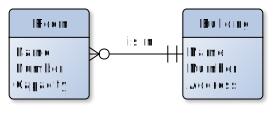
\includegraphics[scale=0.7]{\currentDir/erdRoom2}}%
%
\floatSep%
%
\subfloat[][%
A realization of the \pgls{ERD} given in \cref{fig:erdRoom2} as a logical model that uses only a single table and that violates the \pgls{2NF}.%
\label{fig:violation2nf:model}%
]{\parbox[t]{0.5\linewidth}{\centering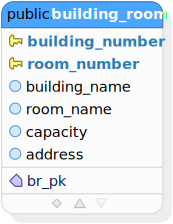
\includegraphics[width=0.4\linewidth]{\currentDir/violation2nf}}}%
%
\caption{An example for a violation of the \glsreset{2NF}\gls{2NF}:~%
The table~\sqlil{building_room} has a composite primary key composed of the room number and building number. %
However, the other attributes each only depend on one part of this primary key.}%
\label{fig:violation2nf}%
\end{figure}%
%
\gitExec{\databasesCodeRepo}{.}{_scripts_/postgres.sh normalization/2nf/violation/generated_sql 01_violation_database_2001.sql}%
%
\gitSQL{\databasesCodeRepo}{normalization/2nf/violation/generated_sql/03_public_building_room_table_5071.sql}{2nf:violation:03_public_building_room_table_5071}{The generated \sql\ code for creating the table \sqlil{building_room} that violates the \pgls{2NF} based on \cref{fig:violation2nf:model}.}%
\gitExec{\databasesCodeRepo}{.}{_scripts_/postgres.sh normalization/2nf/violation/generated_sql 03_public_building_room_table_5071.sql violation}%
%
\gitSQL{\databasesCodeRepo}{normalization/2nf/violation/insert.sql}{normalization:2nf:violation:insert}{%
Inserting some data into the table~\sqlil{building_room} in violation of the \pgls{2NF}.}%
\gitExec{\databasesCodeRepo}{.}{_scripts_/postgres.sh normalization/2nf/violation insert.sql violation}%
%
\gitSQLAndOutput{\databasesCodeRepo}{normalization/2nf/violation}{delete.sql}{violation}{}{}{postgres.sh}{normalization:2nf:violation:delete}{%
First, we select a list of all buildings from the \db, which yields 4~buildings. %
Then we delete the two offices 904a and 904b of Building~53 from our \db. %
This causes a deletion anomaly~(\cref{def:deletionAnomaly}):~all data about Building~53 to disappear. %
So when we select the list of all buildings again, now there are only~3.}%
%
\gitSQLAndOutput{\databasesCodeRepo}{normalization/2nf/violation}{update.sql}{violation}{}{}{postgres.sh}{normalization:2nf:violation:update}{%
We want to see all rooms in South Campus~2. %
Due to some inconsistent spelling~(South Campus~II vs.\ South Campus~2), the first query misses some rooms. %
We then run a modified query, which gives us all the rooms. %
We can also fix the table by updating the corresponding rows, after which the first query also works correctly.%
}%
%
\gitSQLAndOutput{\databasesCodeRepo}{normalization/2nf/violation}{update2.sql}{violation}{}{}{postgres.sh}{normalization:2nf:violation:update2}{%
We want to change the name of Building~36 to \inQuotes{Computer Science Building.} %
While we only want to change one single piece of information, we actually have to update three rows. %
This is an update anomaly~(\cref{def:updateAnomaly}) caused by the violation of the \pgls{2NF} of our design.%
}%
%
\gitExec{\databasesCodeRepo}{.}{_scripts_/postgres.sh normalization/2nf/violation cleanup.sql}%
%
If a table is normalized to the \pgls{2NF}, then all attributes depend on the entire primary key.
This only matters if the primary key is composite, i.e., if it consists of multiple columns.
If a table violates the \pgls{2NF}, then this means that some columns are functionally dependent only on a part of but not the whole primary key.

Let us explore why this can be a bad thing.
Back in \dref{fig:erdRoom1}, we presented an \pgls{ERD} for the room planning subsystem of our teaching management platform.
In \cref{fig:violation2nf:model}, we show only a part of this diagram, namely the two entity types \emph{Room} and \emph{Building}.
As you can see, the two entity types are related based on the \crowsFoot{Room}{OM}{Building}{M1} pattern.
We showed how this pattern can be implemented in \dref{sec:rm:kl}.

Assume that a \db\ designer wanted to cut their losses and decided to just put all the room and building data into a single table.
The result is illustrated in \cref{fig:violation2nf}.
The table~\sqlil{building_room} was designed.
It holds the columns \sqlil{building_number}, \sqlil{room_number}, \sqlil{building_name}, \sqlil{room_name}, \sqlil{capacity}, and \sqlil{address}.
\sqlil{building_number}, \sqlil{room_number}
The \sqlil{building_number} and \sqlil{room_number} are both of type \sqlilIdx{VARCHAR} with a maximum length of 4, as they do not necessarily be numbers but could also be something like~\sqlil{'105b'}.
The type \sqlilIdx{VARCHAR} is for variable-length text strings.
Together, the two columns form the primary key:
Each room in our university is uniquely identified by the building and room number.
There cannot be two different rooms that have the same building and room number.

This design violates the \pgls{2NF} because we have some columns that depend only on a part of the primary key.
The columns \sqlil{building_name} and \sqlil{address} are facts about \sqlil{building_number} alone.
They do not functionally depend on \sqlil{room_number}.

In \cref{lst:2nf:violation:03_public_building_room_table_5071}, we illustrate the \sql\ code that generates the table.
It also creates the columns for the room and building names as well as the address as \sqlilIdx{VARCHAR} with a maximum length of~100.
The capacity for people of the room is an \sqlilIdx{INTEGER} number.
In \cref{lst:normalization:2nf:violation:insert}, we fill the table with some data.
For example, we store the meeting room~(room~305) of Building~36~(the Computer Science Teaching Building), located in South Campus~2.
We also store information about a lecture room in the same building.
We store information about two teaching rooms in the Language Teaching Building in South Campus~1, as some offices in Building~53 of South Campus~2, and some other rooms.

One thing immediately becomes clear when reading these \sqlilIdx{INSERT} statements:
This structure creates a lot of redundancy:
For example, the address of Building~36 is stored three times.
Actually, the name of Building~36 is stored three times as well.
This feels wrong.

With the first query in \cref{lst:normalization:2nf:violation:delete}, we want to extract a list of all buildings from our \db.
We will \sqlilIdx{SELECT} the building number and building name from our table~\sqlil{building_rooms}.
Since these occur several times, we write \sqlilIdx{SELECT DISTINCT}\sqlIdx{DISTINCT} instead of just~\sqlilIdx{SELECT}.
This only returns the unique rows.
The output shows us that we have four buildings in our \db, as expected.

Assume that some time has passed and we decided that Rooms~904a and~904b are no longer used for small-group teaching.
So with the second query in the listing, we delete them from our \db.
We do this by using the \sqlilIdx{DELETE FORM} statement, with the~\sqlilIdx{WHERE} criterion requiring that the building number must be~53 and the room number must be~\sqlil{LIKE '904\%'}\sqlIdx{LIKE}, meaning that it must start with~904 followed by an arbitrary character.
\postgresql\ allows us to also add the \sqlilIdx{RETURNING} statement~\cite{PGDG:PD:RDFMR}, that acts like a \sqlilIdx{SELECT} on the deleted rows.
The output of the command therefore is the building number and room number of the deleted rooms.
We see that, indeed, rooms~904a and 904b of Building~53 are deleted.

We now run the same query giving us the list of buildings again~(as the third query in \cref{lst:normalization:2nf:violation:delete}).
We notice that, by deleting the two rooms in Building~53, we inadvertently also deleted all information about the building.
Its building number, building name, and building address are all lost.
Because they were stored together with the room records.
This is called \emph{deletion anomaly}.%
%
\begin{definition}[Deletion Anomaly]%
\label{def:deletionAnomaly}%
A situation where the deletion of unwanted information causes desired information to be deleted as well is called~\emph{deletion anomaly}~\cite{S2024D:RNDAFDNF}.%
\end{definition}%
%
Well, of course, you may argue that in some cases, that would actually be the desired effect.
For example, in the original model given in \dref{fig:erdRoom1}, the relationship between buildings and rooms was specified as \crowsFoot{Room}{MM}{Building}{M1}.
In this patter, discussed in \dref{sec:rm:mn}, it would be required to delete the building data if all rooms in the building were removed.
The problem is that this deletion also occurs if we try to follow the \crowsFoot{K}{M1}{L}{OM}, where such deletion is not warranted.

\Cref{lst:normalization:2nf:violation:update} illustrates another issue that is encouraged~(but not caused) by a violation of the \pgls{2NF}: inconsistency.
Assume that we wanted to get a list of all rooms available in South Campus~2.
We could fire out the first query given in \cref{lst:normalization:2nf:violation:update}, namely we could simply \sqlilIdx{SELECT} the building number and room number where \sqlil{address = 'South Campus 2'}.
This query only returns a single room, namely room~106 in Building~36.
We know that this is wrong, we definitely entered more than one room for Building~36.
Scrolling back to our insertion script in \cref{lst:normalization:2nf:violation:insert}, we noticed that we sometimes wrote~\sqlil{'South Campus II'} instead of~\sqlil{'South Campus 2'}.
Obviously, for a computer, these are two different things.

The fact that we need to store the same data again and again makes such mistakes more likely.
Whenever a person enters some information into the computer, there is a certain probability that they make an error.
The more often we enter data, the higher the chance that some error is made somewhere.
Violating the \pgls{2NF} forces us to write the same information more often, hence it increases the chance of making an error.
The violating the \pgls{2NF} does not \emph{cause} the error, but it makes it more likely.%
%
\begin{sloppypar}%
Anyway, we can solve the above problem in two ways:
Either we select all rows where \sqlil{address = 'South Campus 2'} \emph{or} \sqlil{address = 'South Campus II'}, as done in the second query.
Or we just fix the incorrectly entered data with an \sqlilIdx{UPDATE} command that sets the building address to \sqlil{'South Campus 2'} if it currently is \sqlil{'South Campus II'}.
We again enrich this query with a \sqlilIdx{RETURNING} statement~\cite{PGDG:PD:RDFMR} which will print out all the rows that were modified with this statement.
After this update, the original query works as well.%
\end{sloppypar}%
%
Finally, let us try to change the name of Building~36 from \inQuotes{CS Teaching Building} to \inQuotes{Computer Science Building.}
This can be done with the query shown in \cref{lst:normalization:2nf:violation:update2}.
We again use an \sqlilIdx{UPDATE} statement applied to our table~\sqlil{building_room}.
This time, we want to modify the rows where \sqlil{address = 'South Campus 2'} and \sqlil{building_number = '36'}.
For all of these rows, we set \sqlil{building_name = 'Computer Science Building'}.
We again use the \sqlilIdx{RETURNING} statement~\cite{PGDG:PD:RDFMR} to print out all the rows that were modified with this statement.
As you can see, this changes three rows.
Notice that we wanted to change only \emph{one} single piece of data.
But we did change \emph{three} rows.%
%
\begin{definition}[Update Anomaly]%
\label{def:updateAnomaly}%
A situation where changing one piece of information requires that multiple rows must be updated is called~\emph{update anomaly}.%
\end{definition}%
%
This anomaly is directly caused by the violation of the~\pgls{2NF}.
And another anomaly results from it as well:%
%
\begin{definition}[Insertion Anomaly]%
A situation where inserting data into the \db\ is not possible because other data is not already there is called~\emph{insertion anomaly}~\cite{S2024D:RNDAFDNF}.%
\end{definition}%
%
For example, it is simply not possible to insert information about a room without inserting information about a building as well.
Of course, in our special case here, this would not make any sense anyway.

In~\cite{K1983ASGTFNFIRDT}, however, another interesting case is presented from the field of warehousing.
The names and addresses of warehouses are stored together with the names and quantities of the products in them.
In a table that violates the \pgls{2NF}, there can be exactly these four columns.
In such a case, it is not possible to create a record for a warehouse if no product is stored in it as well.%
%
\FloatBarrier%
\endhsection%
%
